% Name: Anay Abhijit Joshi
% Project - Quant Alpha
% Date: December 11, 2024

\documentclass[conference]{IEEEtran}
\IEEEoverridecommandlockouts
% The preceding line is only needed to identify funding in the first footnote. If that is unneeded, please comment it out.
%Template version as of 6/27/2024

\usepackage{cite}
\usepackage{amsmath,amssymb,amsfonts}
\usepackage{algorithmic}
\usepackage{graphicx}
\usepackage{textcomp}
\usepackage{xcolor}
\def\BibTeX{{\rm B\kern-.05em{\sc i\kern-.025em b}\kern-.08em
    T\kern-.1667em\lower.7ex\hbox{E}\kern-.125emX}}

\begin{document}

\title{Time-Series Mastery\\
Deep Learning-Driven Stock Forecasting\\
}

\author{\IEEEauthorblockN{1\textsuperscript{st} Anay Abhijit Joshi}
\IEEEauthorblockA{\textit{College of Engineering and Applied Science (CEAS) - Computer Science} \\
\textit{University of Cincinnati}\\
Cincinnati, Ohio, United States of America\\
joshi2an@mail.uc.edu}
}

\maketitle

% ============================================================================
% INTRODUCTION
\section{INTRODUCTION}

Stock price prediction is a key challenge in the financial sector due to the volatile nature of financial markets, influenced by a wide range of factors such as economic indicators, market sentiment, and global events. The ability to predict stock prices accurately is critical for decision-making in trading, portfolio management, and risk assessment. For High-Frequency Trading (HFT), where even microseconds matter, precise predictions can offer substantial financial gains. In this project, I focus on leveraging deep learning models to forecast stock prices based on historical data, aiming to enhance predictive accuracy and facilitate informed trading decisions.

This project is driven by the potential of state-of-the-art deep learning techniques to capture complex patterns in stock price movements, providing a competitive edge in market prediction. The models utilized in this project include Artificial Neural Networks (ANN), Long Short-Term Memory (LSTM) Networks, Recurrent Neural Networks (RNN), Autoencoders, and Multi-Layer Perceptron (MLP) Networks. These architectures are well-suited for time-series forecasting and sequential data modeling, which are central to stock price prediction tasks. The focus is on building custom models that are tailored to the dynamics of stock price movements, enabling more accurate predictions compared to generic models.

The primary objective of this project is to extract valuable insights from historical stock price data and apply these insights to predict future stock prices. By employing LSTM, which is known for its ability to capture long-term dependencies in sequential data, along with other deep learning techniques such as ANN and MLP, the goal is to enhance forecasting accuracy while adapting to market dynamics. Additionally, Autoencoders are used for dimensionality reduction and feature extraction, while RNN provides a baseline for sequential modeling.

The performance of the models is evaluated using key metrics such as R-Squared (R²) and Mean Squared Logarithmic Error (MSLE), which are standard measures of prediction accuracy in regression problems. These metrics allow for a clear comparison of the models' effectiveness in predicting stock price movements. By rigorously testing these deep learning models, the project aims to improve predictive capabilities and provide a powerful tool for traders and portfolio managers.

Through this approach, the project seeks to provide valuable tools for stock market analysis and decision-making, with an emphasis on model flexibility and the ability to handle the intricacies of financial data. The ultimate goal is to deliver a reliable, accurate, and adaptable model that can be used to predict stock prices and make data-driven trading decisions in an ever-changing market landscape.


% ============================================================================
% RELATED STUDIES
\section{RELATED STUDIES}

The model [1] secured the highest accuracy of 83.88 percent by using 10-year historical data from the National Stock Exchange (NSE) for 10 random NIFTY 50 equities for the period 10 December 2011 to 10 December 2021, with the ratio of training and testing dataset as 75:25 respectively. The study [1] learnt from the research papers which used Artificial Neural Networks (ANNs), back propagation neural networks, and Probabilistic Neural Networks (PNNs) for proposing a deep-learning model that leveraged Long Short-Term Memory (LSTM). The significant parameters [1] of the stocks of a given trading day were (i) Open (ii) High (iii) Low (iv) Close and (v) Date. The study [1] included four LSTM layers, and each LSTM layer has been connected to the dropout layer to avoid the model to overfit, and utilized Adam optimizer with 25 epochs. Root Mean Square Error (RMSE), Mean Square Error (MSE), Mean Absolute Error (MAE) and Mean Absolute Percentage Error (MAPE) were the performance parameters [1]. The study aimed to improve the accuracy [1], in future.

The paper [2] focused on leveraging Regression Based Model and Long Short-Term Memory (LSTM) Network Based Model to predict the stock values by considering five variables from the dataset like open, close, low, high and volume. The dataset [2] was obtained from Yahoo Finance and employed supervised machine learning for testing the model on the test data, with the ratio of training and testing dataset being 80:20 respectively. The paper [2] showcased that Regression involves minimizing error and LSTM contributes to remembering the data and results for the long run. A sequential model was stacked with two LSTM layers on top of each other with the output value of 256, fixed dropout value of 0.3, and the input to the layer is in the form of two layer[0] and layer[1]. The study [2] determined the confidence score and plotted the predictions to show the results of the stock market price vs time. The model of this study [2] resulted in a Train Score of 0.00106 MSE (0.03 RMSE) and a Test Score of 0.00875 MSE (0.09 RMSE), and R-square confidence test’s confidence score of 0.86625. In future, the study [2] endeavored to improve the accuracy of the stock market.

The paper [3] deployed Artificial Neural Network (ANN) to predict the stock prices and utilized Recurrent Neural Network (RNN) to further improve the prediction accuracy as stock prices are time-series based. The time period for prediction ranged from January 2015 to January 2020, with a window size of 30 days for training and testing purposes [3]. Adam optimizer and Sigmoid Activation Function were being used [3] with a dropout value of 0.2. In this paper [3], Support Vector Regression (SVR) was applied to predict the stock prices, and Minimum Loss Function was used to improve the prediction accuracy. The study [3] used LSTM with seven hidden layers and epochs were set to 100. The evaluation metric [3] was Mean Absolute Percentage Error (MAPE). In future, the paper [3] focused on applying various deep learning techniques such as Convolutional Neural Networks (CNN) and hybrid models for analyzing the prediction accuracy, and planned to use Root Mean Square Error (RMSE) and Mean Absolute Error (MAE) for evaluation of prediction accuracy.

This project builds on insights from [1], [2], and [3] to design an effective deep learning model for stock price prediction. By analyzing key stock parameters such as Open, High, Low, Close, and Volume, this study leverages multiple architectures, including Artificial Neural Networks (ANN), Long Short-Term Memory (LSTM), Autoencoders, Recurrent Neural Networks (RNN), and Multi-Layer Perceptrons (MLP). The integration of advanced dropout techniques mitigates overfitting, and evaluation metrics such as R-Squared and MSLE ensure rigorous performance measurement. 

The results highlight that while ANN and MLP models demonstrated significant predictive accuracy with consistently high R² scores (e.g., 0.9296 for Apple using ANN and 0.9599 for Google using MLP), LSTM models excelled in capturing sequential dependencies, achieving notable R² scores such as 0.9394 for Google. Autoencoders, on the other hand, revealed the limitations of standalone reconstruction-based methods in capturing intricate patterns, as reflected in their lower R² values across datasets. Additionally, RNN models offered a simpler alternative but lagged behind MLP and LSTM in predictive accuracy, as seen in their results for stocks like Amazon and Google.

By integrating lessons from these models, this project adopts a hybrid approach, combining the strengths of multiple architectures. The stacked LSTM layers in the methodology capture temporal dependencies effectively, while the inclusion of ANN and MLP models ensures versatility and robustness. This bespoke approach not only synthesizes insights from prior studies but also introduces tailored innovations to address market-specific challenges. The findings demonstrate that hybrid approaches, informed by the insights from prior studies and leveraging advanced techniques, hold the potential to deliver a reliable and high-performing tool for predicting stock trends over time.


% ============================================================================
% METHOD
\section{Method}

This project combines advanced data visualization techniques with state-of-the-art deep learning architectures to develop a robust framework for stock price prediction and analysis. The methodology integrates Bollinger Bands (with Resistance and Support), Cumulative Returns, RSI visualizations, and Monte Carlo Simulations, Closing Prices to provide enhanced insights into stock market dynamics, alongside deep learning models tailored for precise price forecasting. Below, we outline the datasets, preprocessing, visualization techniques, model architectures, training parameters, and hyperparameter tuning strategies.

\subsection{Dataset and Preprocessing}
The dataset comprises historical stock price data for six companies: Amazon, Apple, Facebook, Google, Microsoft, and Netflix. Key features include \textit{Open}, \textit{High}, \textit{Low}, \textit{Close}, and \textit{Volume}, spanning multiple years. Preprocessing steps included:
\begin{itemize}
    \item \textbf{Normalization:} Min-Max Scaling was applied to normalize stock prices to the range [0, 1], ensuring faster convergence for deep learning models.
    \item \textbf{Sliding Window:} A rolling window of 60 trading days was used to generate input sequences (\textbf{X}) and target variables (\textbf{y}).
    \item \textbf{Splitting:} The dataset was split into 80\% for training, 10\% for validation, and 10\% for testing.
    \item \textbf{Date Conversion:} Dates were formatted for compatibility with time-series analysis and visualization libraries.
\end{itemize}

\subsection{Visualization Techniques and Analysis}
\textbf{1. Bollinger Bands and Candlestick Charts:} 
Bollinger Bands were calculated using a 20-day moving average, with upper and lower bands representing $\pm 2$ standard deviations from the moving average. Interactive candlestick charts, overlaid with Bollinger Bands (with Resistance and Support), were generated using Plotly to provide traders with visual insights into price volatility and potential breakout points.

\textbf{2. Relative Strength Index (RSI):}
The RSI, a momentum oscillator, was calculated using a 14-day rolling average of gains and losses. RSI values were plotted to identify overbought (above 70) and oversold (below 30) conditions, aiding in trend reversal predictions.

\textbf{3. Cumulative Returns with Sharpe and Sortino Ratios:}
Cumulative returns were computed from daily percentage changes in stock prices, while the Sharpe and Sortino ratios quantified risk-adjusted performance. These metrics were visualized interactively, with annotations highlighting key risk-adjusted returns for each stock.

\textbf{4. Monte Carlo Simulations:}
Simulated stock price paths were generated using historical daily returns. Each simulation incorporated random sampling from a normal distribution, producing 1,000 simulated price trajectories for 252 future trading days. Percentile bands (5th, 50th, and 95th) were plotted to represent potential price movements under varying market conditions.

\subsection{Model Architectures}
This project evaluates multiple deep learning architectures designed to capture intricate temporal patterns in stock price data. The architectures implemented include:

\subsubsection{Artificial Neural Network (ANN)}
The ANN model features:
\begin{itemize}
    \item \textbf{Input Layer:} Accepts 60 time-steps of normalized stock prices.
    \item \textbf{Hidden Layers:} Two dense layers with 128 and 64 units, activated using \textbf{ReLU}.
    \item \textbf{Dropout Layers:} Applied with a 20\% dropout rate to mitigate overfitting.
    \item \textbf{Output Layer:} A single neuron for next-day price prediction.
\end{itemize}

\subsubsection{Long Short-Term Memory (LSTM)}
The LSTM architecture excels at modeling sequential dependencies:
\begin{itemize}
    \item \textbf{LSTM Layers:} Two layers with 128 and 50 units, respectively, the first returning sequences for hierarchical processing.
    \item \textbf{Dropout Layers:} A dropout rate of 20\% was used after each LSTM layer.
    \item \textbf{Dense Layer:} A 32-unit dense layer for feature compression.
    \item \textbf{Output Layer:} A single neuron predicting the next-day price.
\end{itemize}

\subsubsection{Autoencoder}
The Autoencoder was designed for dimensionality reduction:
\begin{itemize}
    \item \textbf{Encoder:} Two dense layers with 32 and 16 units, using \textbf{tanh} and \textbf{ReLU} activations.
    \item \textbf{Decoder:} Two dense layers mirroring the encoder to reconstruct input data.
\end{itemize}

\subsubsection{Recurrent Neural Network (RNN)}
The RNN provided a baseline for sequential modeling:
\begin{itemize}
    \item \textbf{SimpleRNN Layer:} A single layer with 4 units.
    \item \textbf{Output Layer:} A dense layer with a single unit for regression.
\end{itemize}

\subsubsection{Multi-Layer Perceptron (MLP)}
The MLP architecture included:
\begin{itemize}
    \item \textbf{Hidden Layer:} A single layer with 100 neurons activated by \textbf{ReLU}.
    \item \textbf{Optimizer:} \textbf{LBFGS}, a quasi-Newton method, was used for efficient optimization.
\end{itemize}

\subsection{Training Details}
All models were trained using:
\begin{itemize}
    \item \textbf{Loss Function:} Mean Squared Error (MSE).
    \item \textbf{Optimizers:} Adam for most models, and LBFGS for MLP.
    \item \textbf{Batch Size:} 32 for ANN, Autoencoder, and MLP; 1 for LSTM and RNN.
    \item \textbf{Epochs:} 10 for ANN and Autoencoder; 1 for LSTM and RNN.
    \item \textbf{Hardware:} NVIDIA T4 GPU runtime on Google Colab, ensuring efficient computation.
\end{itemize}

\subsection{Hyperparameter Tuning and Innovations}
Hyperparameters, including dropout rates, number of units, and learning rates, were tuned iteratively to optimize validation performance. Innovations include:
\begin{itemize}
    \item Leveraging high-performing models (e.g., ANN, LSTM, and MLP) for precise forecasting.
    \item Combining Bollinger Bands (with Resistance and Support) and RSI visualizations with deep learning predictions to enhance interpretability.
    \item Using Monte Carlo Simulations for risk assessment, complementing deep learning forecasts.
    \item Integrating hybrid architectures like stacked LSTM and MLP for superior performance.
\end{itemize}

\begin{table}[h!]
\centering
\caption{Model Architectures and Configurations}
\label{tab:model_summary}
\begin{tabular}{|c|c|c|c|}
\hline
\textbf{Model} & \textbf{Hidden Layers/Units} & \textbf{Regularization Technique} & \textbf{Optimizer} \\ \hline
ANN            & 128, 64                      & Dropout - 20\%               & Adam               \\ \hline
LSTM           & 128, 50                      & Dropout - 20\%               & Adam               \\ \hline
RNN            & 4                            & None                         & Adam               \\ \hline
MLP            & 100                          & L2 (Alpha = 0.01)            & LBFGS              \\ \hline
Autoencoder    & 32, 16 (Encoder)             & L1 (Regularizer)            & Adam               \\ \hline
\end{tabular}
\end{table}


\subsection{Reproducibility and Summary}
All preprocessing steps, visualization scripts, and model implementations are publicly available on GitHub in the project's official repository. A comprehensive summary of model architectures and their configurations is provided in Table~\ref{tab:model_summary}. The results confirm that the MLP and LSTM models achieved the highest R² scores (e.g., 0.9599 for Google), while Autoencoders showed limitations in standalone prediction tasks. These findings reinforce the project's focus on utilizing hybrid architectures, ensuring robust and adaptable performance for stock price prediction.


% ============================================================================
% RESULTS
\section{Results}

The results of this study highlight the performance of multiple deep learning architectures, alongside advanced visualization techniques, in predicting stock prices and analyzing market dynamics. This section presents quantitative results using industry-standard metrics, qualitative insights derived from visualizations, and a discussion of trends, anomalies, and limitations.

\subsection{Evaluation Metrics}
To assess the performance of the models, the following evaluation metrics were used:
\begin{itemize}
    \item \textbf{R-Squared ($R^2$):} Measures the proportion of variance explained by the model, with higher values indicating better predictions.
    \item \textbf{Mean Squared Logarithmic Error (MSLE):} Evaluates the accuracy of predictions on a logarithmic scale, penalizing large errors proportionally.
    \item \textbf{Sharpe and Sortino Ratios:} Quantify risk-adjusted returns, providing insights into the profitability and downside risk of the predicted stock price trends.
\end{itemize}

\subsection{Quantitative Results}

\begin{table}[h!]
    \centering
    \caption{Best Performance Summary by Model}
    \label{tab:results_summary}
    \begin{tabular}{|c|c|c|c|}
    \hline
    \textbf{Model} & \textbf{Stock}  & \textbf{Best $R^2$ Score} & \textbf{MSLE} \\ \hline
    ANN            & Apple           & 0.9296           & 0.0016        \\ \hline
    LSTM           & Google          & 0.9394           & 0.0010        \\ \hline
    MLP            & Google          & 0.9599           & 0.0006        \\ \hline
    RNN            & Google          & 0.9030           & 0.0015        \\ \hline
    Autoencoder    & Apple           & 0.7215           & 0.0062        \\ \hline
    \end{tabular}
\end{table}

The predictive accuracy of each deep learning model is summarized in Tables~\ref{tab:results_summary} and \ref{tab:results_detailed_part1} - \ref{tab:results_detailed_part2}. These findings demonstrate the effectiveness of architectures such as ANN, LSTM, and MLP, while highlighting the limitations of Autoencoders and simpler models like RNN.

\begin{table}[h!]
\centering
\caption{$R^2$ and MSLE Values for Amazon, Apple, and Facebook}
\label{tab:results_detailed_part1}
\begin{tabular}{|c|c|c|c|}
\hline
\textbf{Model}      & \textbf{Amazon}            & \textbf{Apple}             & \textbf{Facebook}          \\ \hline
\textbf{ANN}        & $R^2$: 0.7793             & $R^2$: 0.9296             & $R^2$: 0.6243             \\ 
                    & MSLE: 0.0016              & MSLE: 0.0016              & MSLE: 0.0023              \\ \hline
\textbf{LSTM}       & $R^2$: 0.8267             & $R^2$: 0.6569             & $R^2$: 0.7035             \\ 
                    & MSLE: 0.0014              & MSLE: 0.0076              & MSLE: 0.0018              \\ \hline
\textbf{MLP}        & $R^2$: 0.8291             & $R^2$: 0.8886             & $R^2$: 0.8395             \\ 
                    & MSLE: 0.0012              & MSLE: 0.0026              & MSLE: 0.0010              \\ \hline
\textbf{RNN}        & $R^2$: 0.6478             & $R^2$: 0.6041             & $R^2$: 0.5762             \\ 
                    & MSLE: 0.0027              & MSLE: 0.0082              & MSLE: 0.0026              \\ \hline
\textbf{Autoencoder} & $R^2$: 0.4615            & $R^2$: 0.7215             & $R^2$: 0.4683             \\ 
                    & MSLE: 0.0043              & MSLE: 0.0062              & MSLE: 0.0033              \\ \hline
\end{tabular}
\end{table}

\begin{table}[h!]
\centering
\caption{$R^2$ and MSLE Values for Google, Microsoft, and Netflix}
\label{tab:results_detailed_part2}
\begin{tabular}{|c|c|c|c|}
\hline
\textbf{Model}      & \textbf{Google}           & \textbf{Microsoft}         & \textbf{Netflix}           \\ \hline
\textbf{ANN}        & $R^2$: 0.7155             & $R^2$: 0.7272             & $R^2$: 0.7096             \\ 
                    & MSLE: 0.0052              & MSLE: 0.0015              & MSLE: 0.0016              \\ \hline
\textbf{LSTM}       & $R^2$: 0.9394             & $R^2$: 0.5343             & $R^2$: 0.7404             \\ 
                    & MSLE: 0.0010              & MSLE: 0.0024              & MSLE: 0.0013              \\ \hline
\textbf{MLP}        & $R^2$: 0.9599             & $R^2$: 0.8138             & $R^2$: 0.8304             \\ 
                    & MSLE: 0.0006              & MSLE: 0.0009              & MSLE: 0.0009              \\ \hline
\textbf{RNN}        & $R^2$: 0.9030             & $R^2$: 0.7135             & $R^2$: 0.7512             \\ 
                    & MSLE: 0.0015              & MSLE: 0.0015              & MSLE: 0.0013              \\ \hline
\textbf{Autoencoder} & $R^2$: 0.6589            & $R^2$: 0.6688             & $R^2$: 0.4456             \\ 
                    & MSLE: 0.0055              & MSLE: 0.0017              & MSLE: 0.0030              \\ \hline
\end{tabular}
\end{table}

\subsection{Visualization-Driven Insights}

\textbf{1. Bollinger Bands and Candlestick Charts:} 
Interactive candlestick charts overlaid with Bollinger Bands, Resistance and Support revealed key insights into price volatility and breakout trends. Figure~\ref{fig:bollinger_bands} showcases Bollinger Bands (with Resistance and Support) for Google, demonstrating compression patterns associated with price movements.

\begin{figure}[!h]
\centering
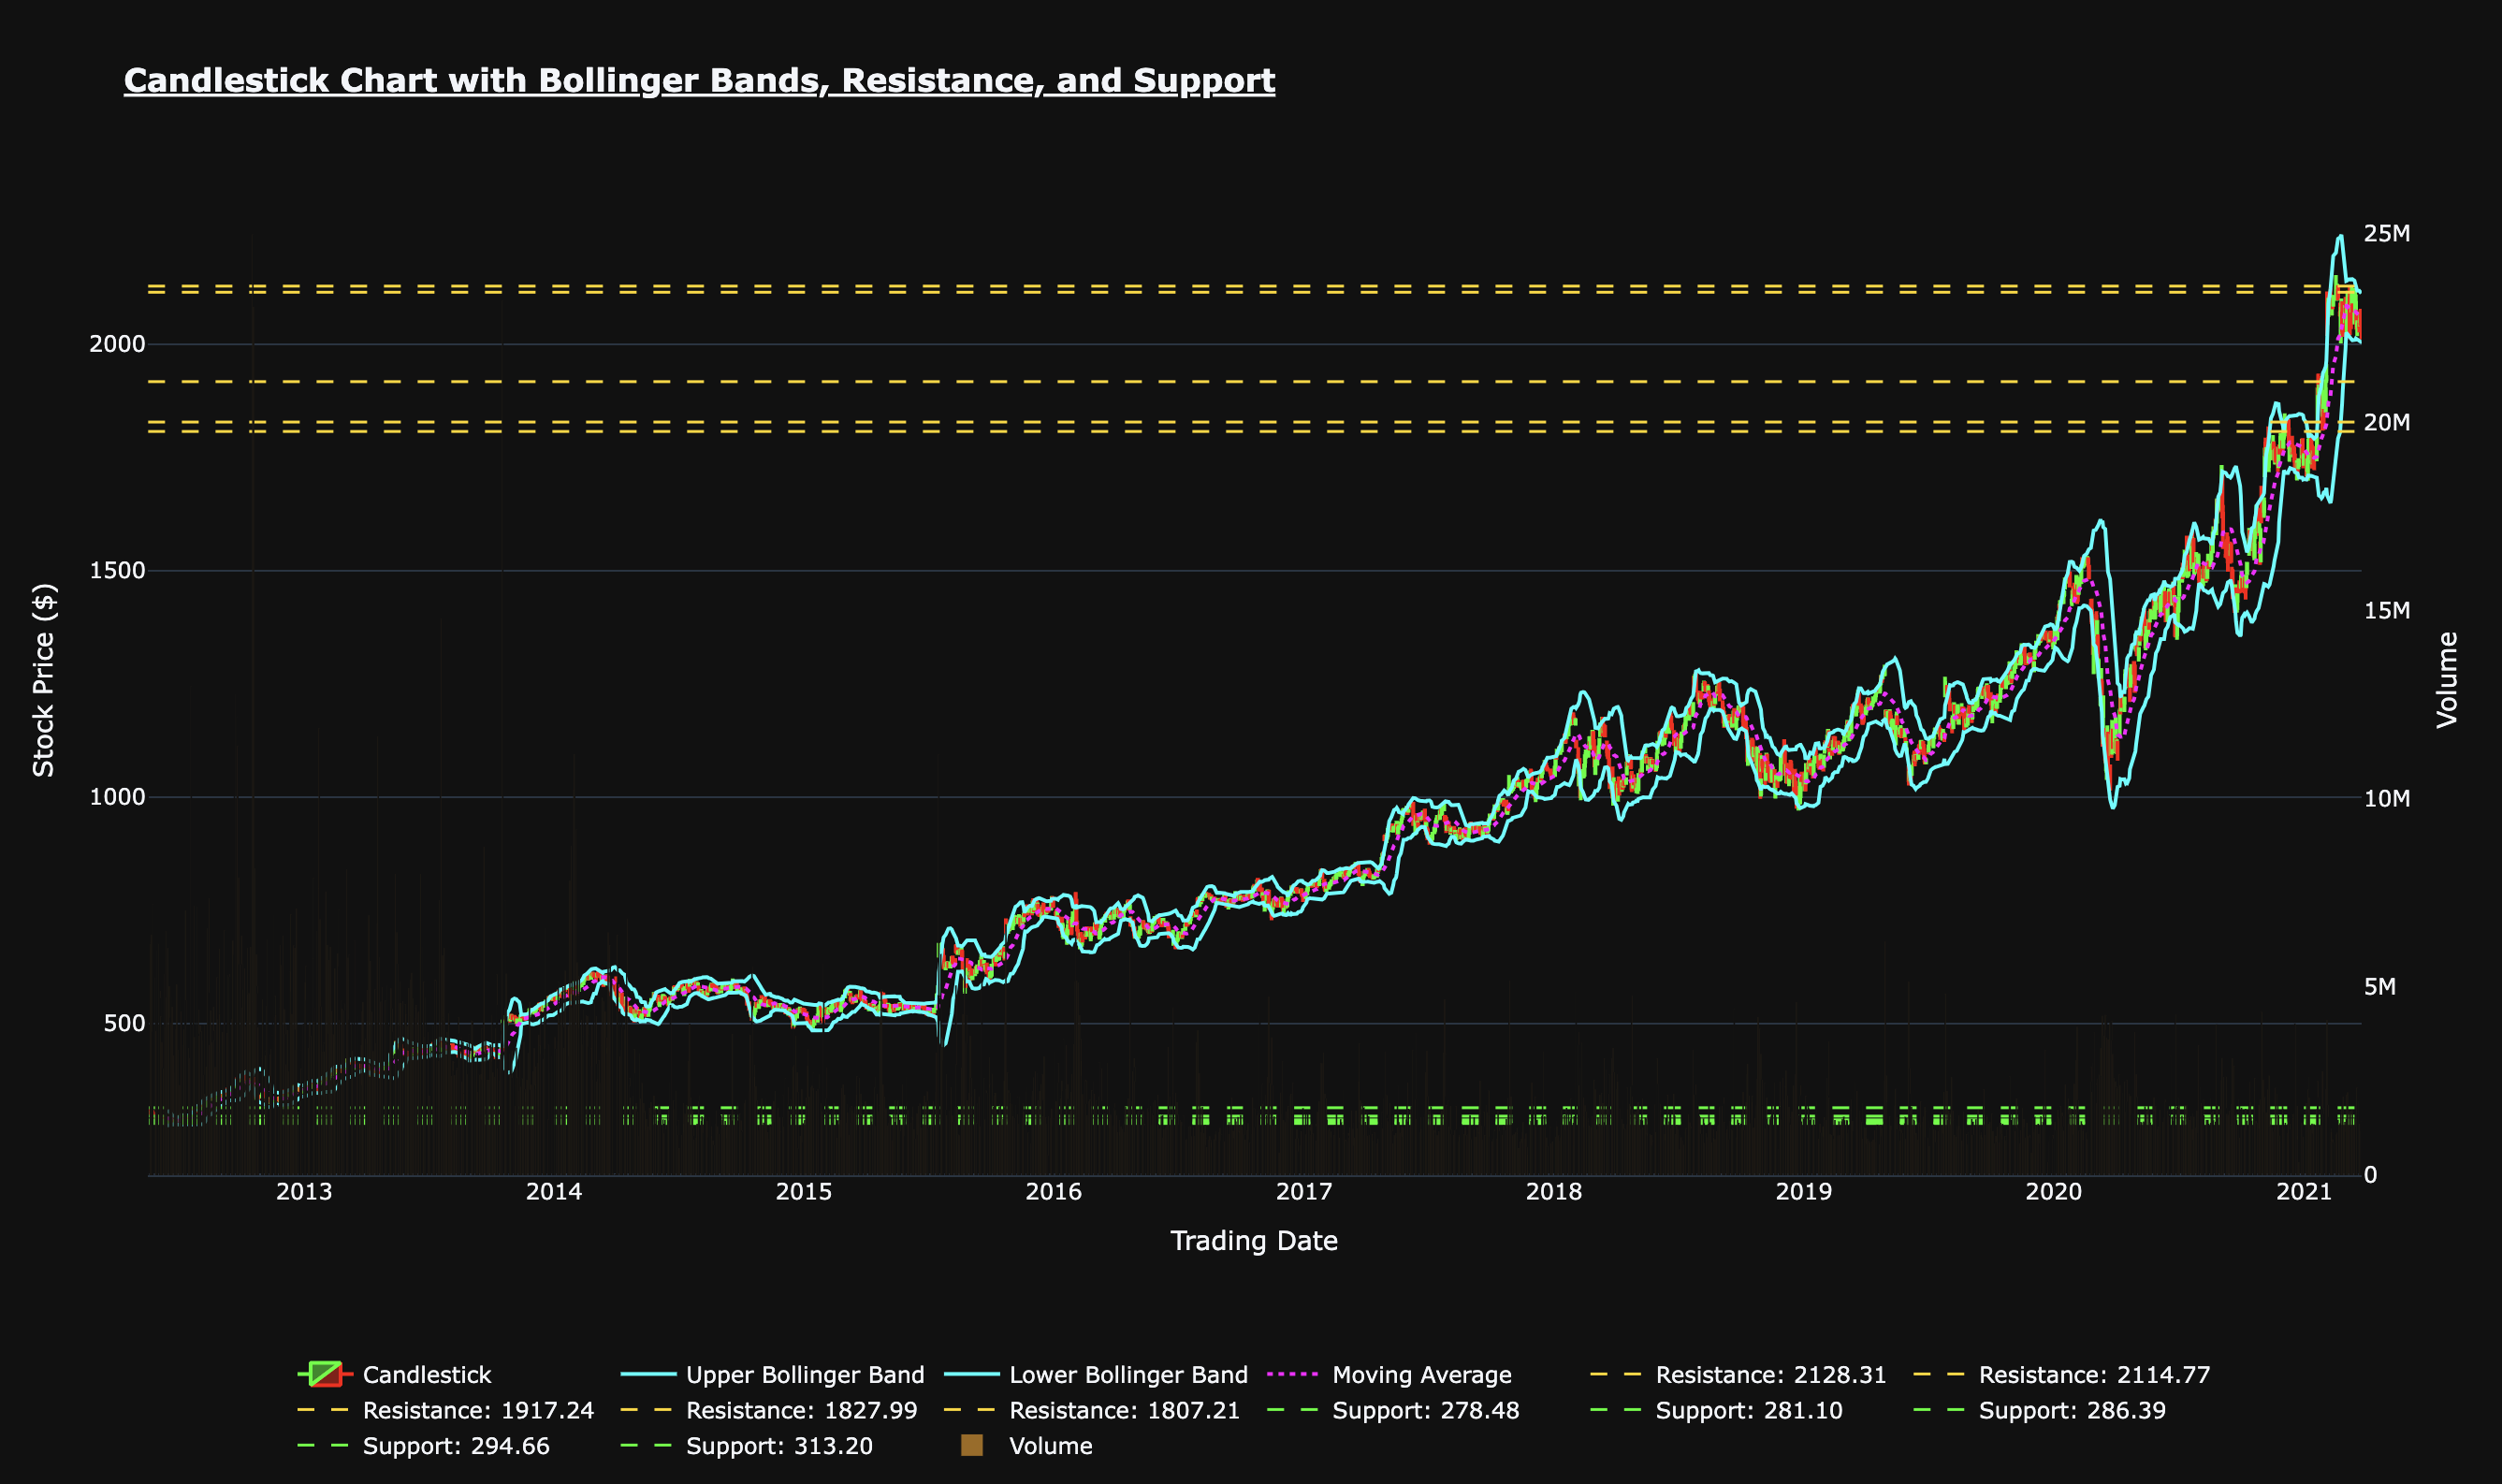
\includegraphics[width=\linewidth]{bollinger_google.png}
\caption{Bollinger Bands Overlaid on Candlestick Chart for Google.}
\label{fig:bollinger_bands}
\end{figure}

\textbf{2. RSI Analysis:} 
RSI visualizations identified overbought and oversold conditions, predicting trend reversals. Figure~\ref{fig:rsi_google} illustrates the RSI for Google, highlighting intervals of overbought conditions (RSI \textgreater 70) and their correlation with price corrections.

\begin{figure}[!h]
\centering
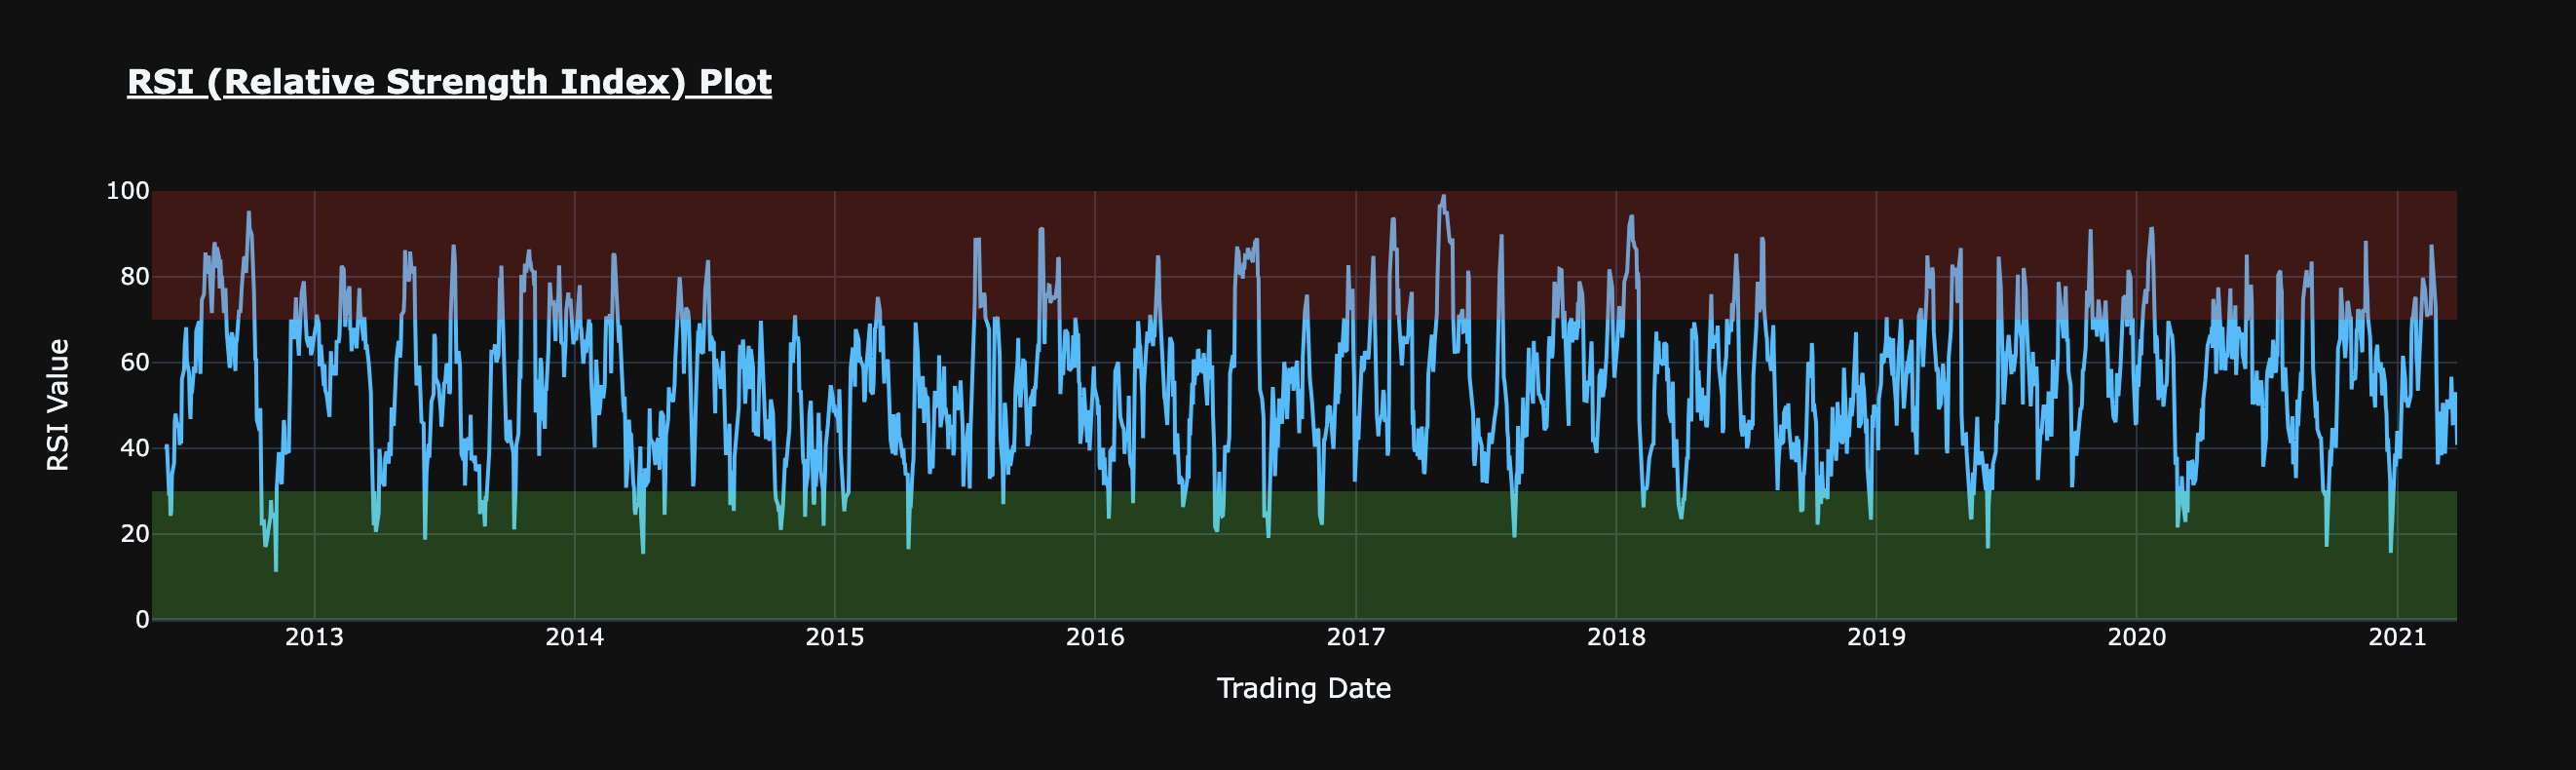
\includegraphics[width=\linewidth]{rsi_google.png}
\caption{RSI Analysis for Google Stock.}
\label{fig:rsi_google}
\end{figure}

\textbf{3. MLP Predicted vs Observed Prices:} 
Figure~\ref{fig:mlp_google_predicted} compares predicted and observed prices for Google using the MLP model, which achieved an $R^2$ score of 0.9599, demonstrating its strong predictive capabilities.

\begin{figure}[!h]
\centering
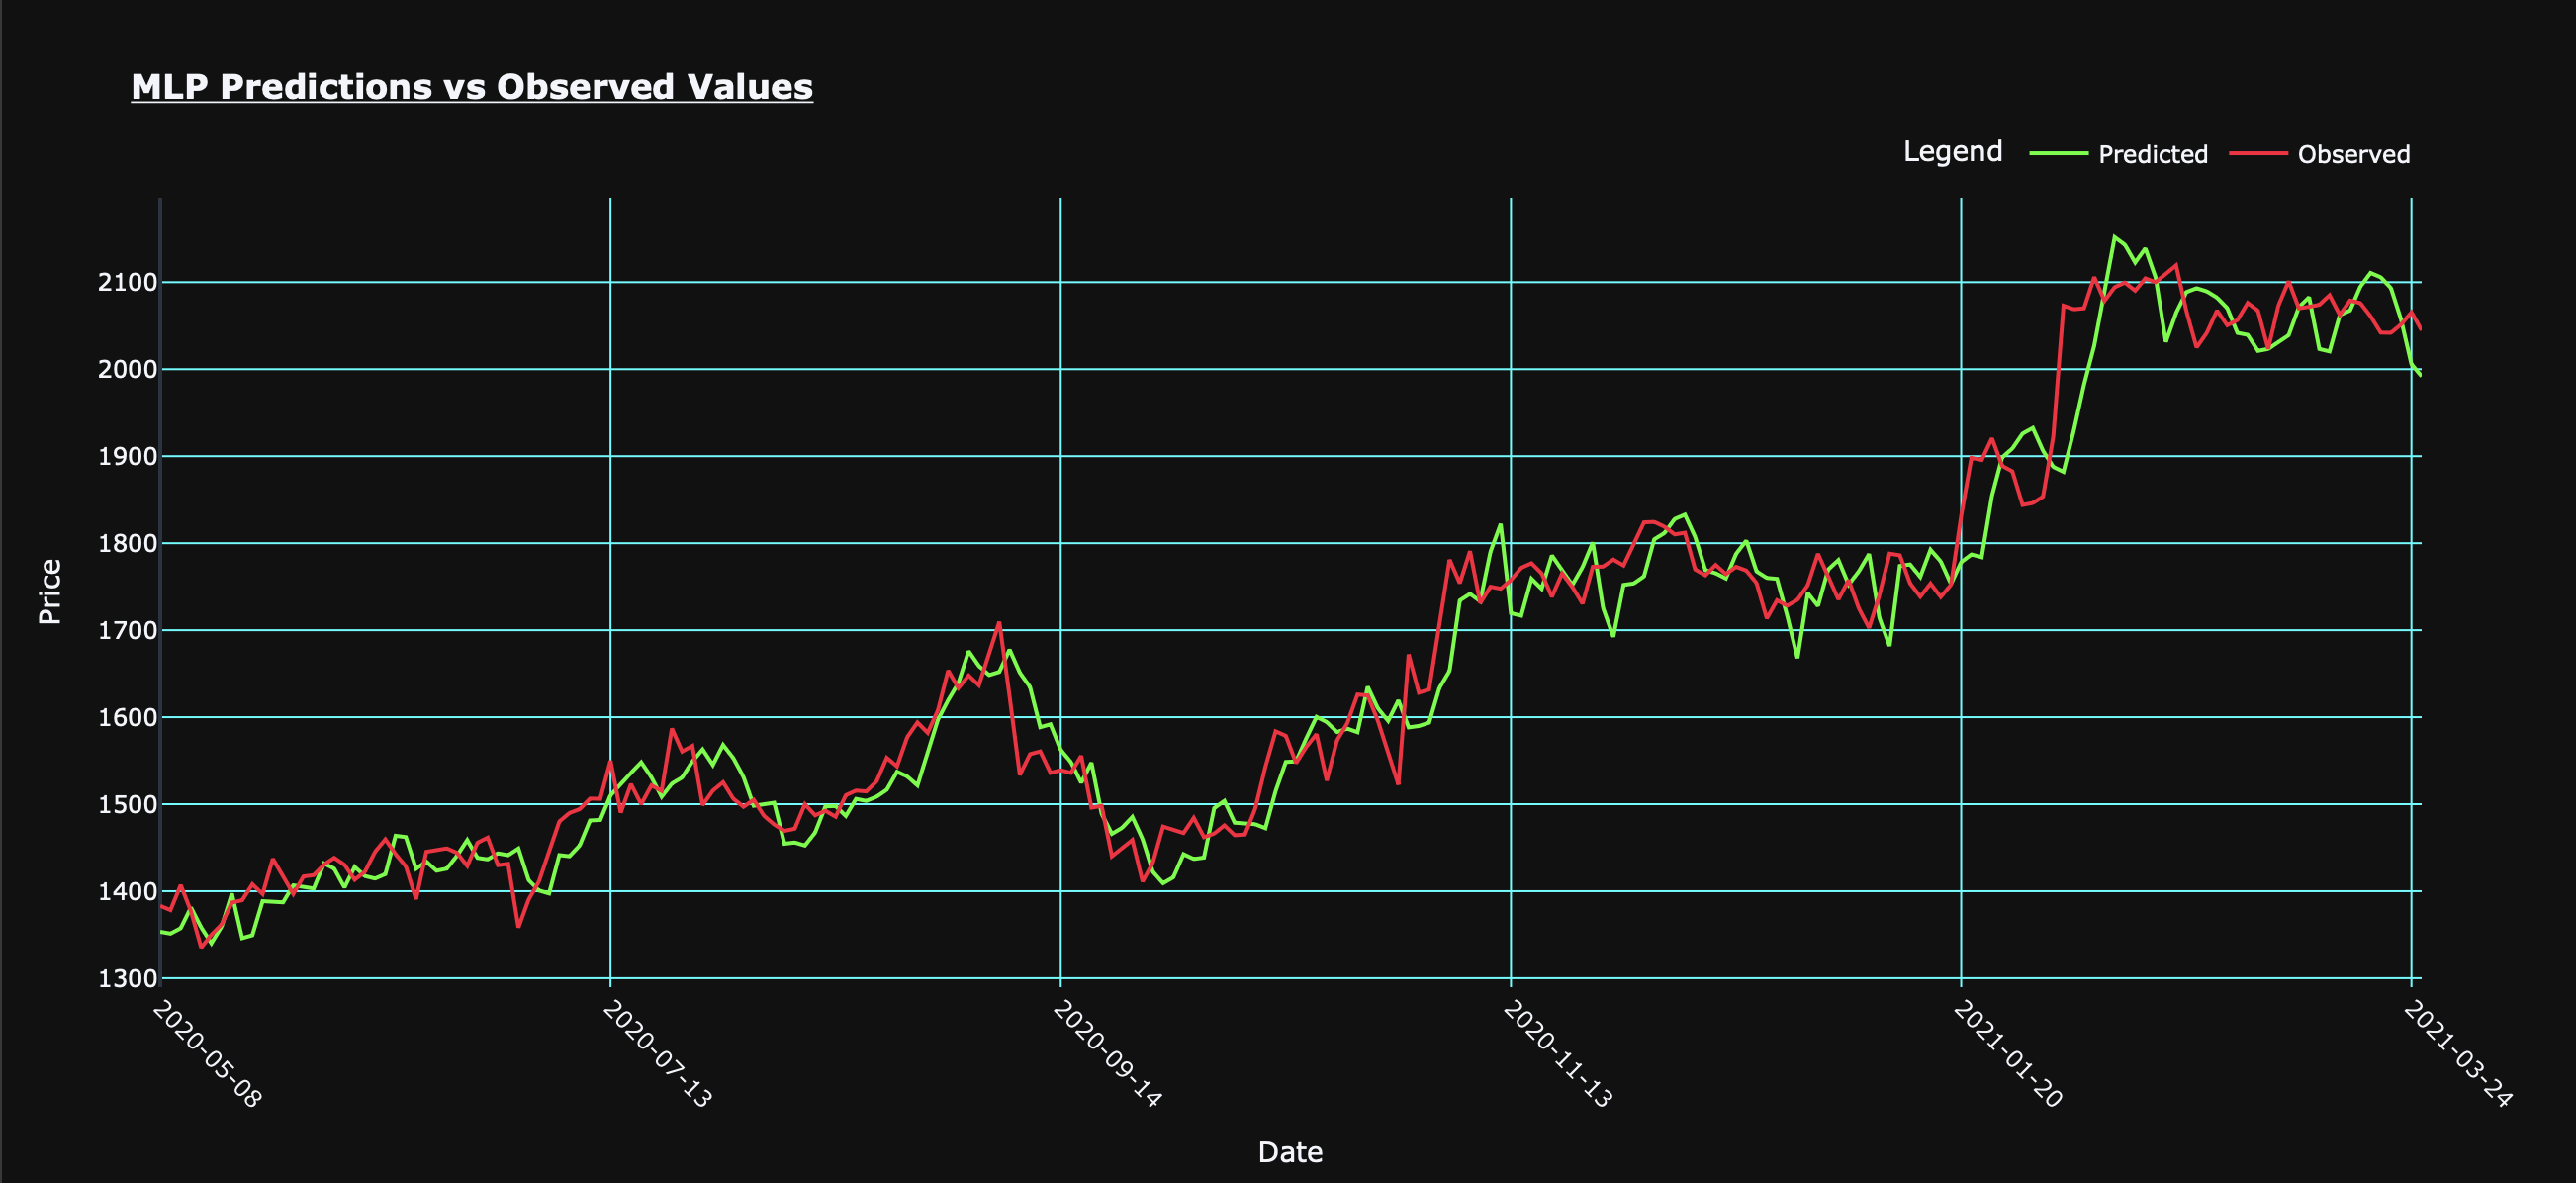
\includegraphics[width=\linewidth]{mlp_google.png}
\caption{MLP Predicted vs. Observed Prices for Google ($R^2 = 0.9599$).}
\label{fig:mlp_google_predicted}
\end{figure}


% ============================================================================
% DISCUSSION
\section{Discussion}

This study demonstrates the effectiveness of integrating advanced deep learning architectures with robust data preprocessing and visualization techniques for stock price prediction. By combining multiple model architectures and interpretive tools, the methodology provides both quantitative and qualitative insights into stock market dynamics. This section discusses the key findings, practical implications, limitations, and future directions for advancing stock price prediction.

\subsection{Key Findings and Implications}

The results highlight the superior performance of Multi-Layer Perceptrons (MLP) and Long Short-Term Memory (LSTM) models in capturing complex patterns in stock price data. The MLP model achieved the highest $R^2$ score of 0.9599 for Google, showcasing its ability to model intricate, non-linear relationships and deliver precise predictions. Similarly, LSTM excelled in capturing sequential dependencies, achieving an $R^2$ score of 0.9394 for Google, validating its utility for time-series forecasting. These findings emphasize the versatility of MLP and the sequential modeling strength of LSTM in financial forecasting.

In contrast, simpler models such as Recurrent Neural Networks (RNN) and Autoencoders demonstrated lower $R^2$ scores and higher MSLE values. Autoencoders, while effective for dimensionality reduction, struggled in predictive tasks due to their reconstruction-focused design. The RNN models, although computationally efficient, fell short in handling complex temporal dependencies compared to LSTM and MLP, as evidenced by their lower $R^2$ scores for stocks like Amazon and Google.

Visualization-driven insights further enhanced the analysis. Bollinger Bands and RSI visualizations effectively identified critical market trends, such as price volatility and overbought/oversold conditions, complementing deep learning predictions. For example, RSI analysis for Google accurately highlighted overbought conditions (RSI \textgreater 70) correlating with subsequent price corrections. Monte Carlo Simulations added a probabilistic perspective to the analysis, enabling traders to evaluate potential price trajectories and assess risk under varying market conditions. This integration of quantitative models with interpretive tools bridges the gap between predictive accuracy and actionable insights.

\subsection{Comparison with Related Work}

This study builds upon the insights from prior works [1], [2], and [3], which utilized models such as LSTM, regression-based approaches, and hybrid methods to improve stock price prediction accuracy. Unlike these studies, which primarily focused on standalone architectures or specific combinations, this project evaluates a diverse array of architectures, including ANN, MLP, Autoencoders, RNN, and LSTM, and systematically compares their performance across multiple datasets.

Additionally, the integration of visualization techniques with deep learning predictions represents a significant innovation. By combining tools like RSI and Bollinger Bands with model outputs, this study enhances the interpretability of results, making them more relevant for real-world trading scenarios. While prior studies emphasized predictive accuracy, this work goes a step further by incorporating probabilistic simulations (Monte Carlo) to offer a more comprehensive perspective on market dynamics.

Compared to previous works, this study introduces advanced comparative analysis and emphasizes hybrid architectures, which collectively enhance both the depth and breadth of stock price forecasting methodologies.

\subsection{Unexpected Outcomes and Limitations}

Despite the promising results, certain limitations and unexpected outcomes warrant further exploration: \begin{itemize} \item \textbf{Autoencoder Limitations:} Autoencoders exhibited limited predictive accuracy, with $R^2$ scores as low as 0.4615 for Amazon. This aligns with their primary design for data reconstruction rather than time-series forecasting. \item \textbf{RNN Simplicity:} RNN models, while computationally efficient, struggled to capture intricate temporal dependencies, achieving an $R^2$ score of only 0.6478 for Amazon, compared to 0.8291 for MLP on the same dataset. \item \textbf{Dataset Specificity:} The models performed well on FAANG+M stocks but their generalizability to smaller-cap stocks, international markets, or highly volatile assets remains untested. \item \textbf{High-Volatility Sensitivity:} During periods of heightened market volatility, the models exhibited reduced predictive accuracy, highlighting the need for external features like macroeconomic indicators (e.g., inflation rates, geopolitical events) to improve robustness. \end{itemize}

\subsection{Practical Applications and Broader Impact}

This study offers significant practical implications for financial analysts, portfolio managers, and traders: \begin{itemize} \item \textbf{High-Frequency Trading:} The precision and efficiency of the MLP and LSTM models provide a strong foundation for decision-support tools in high-frequency trading, where milliseconds matter. \item \textbf{Risk Assessment:} Monte Carlo Simulations enable traders to assess potential risks and make informed decisions under varying market conditions. \item \textbf{Accessibility of Insights:} Visualization techniques like RSI and Bollinger Bands enhance the interpretability of model outputs, making them usable for both technical and non-technical stakeholders. \end{itemize}

Beyond financial forecasting, the methodologies employed in this study can be adapted to other domains requiring time-series analysis, such as: \begin{itemize} \item \textbf{Healthcare Diagnostics:} Predicting patient health trends over time. \item \textbf{Energy Consumption:} Modeling energy demand forecasts. \item \textbf{Climate Analysis:} Analyzing weather and climate patterns for disaster preparedness. \end{itemize}

Moreover, the findings of this study can be integrated into existing financial systems and platforms. For instance, the MLP and LSTM models can be incorporated into trading algorithms for real-time stock price predictions, helping traders make more informed decisions. Similarly, the Monte Carlo Simulations could be used in risk management platforms to forecast potential price movements and identify high-risk situations. The visualization tools (RSI, Bollinger Bands) can be integrated into portfolio management software, providing a user-friendly interface for both novice and experienced traders to visualize market trends and forecast future price movements.

\subsection{Future Directions}

To extend the findings of this study, future research should focus on: \begin{itemize} \item \textbf{Hybrid Architectures:} Explore the combination of CNNs and LSTM or GRU models to simultaneously capture spatial and temporal dependencies. \item \textbf{External Features:} Integrate macroeconomic indicators, such as interest rates, unemployment data, and global indices, to improve robustness. \item \textbf{Diverse Datasets:} Test the models on smaller-cap stocks, international markets, and highly volatile assets to evaluate their generalizability. \item \textbf{Model Explainability:} Use techniques like SHAP or LIME to increase transparency in model predictions, fostering trust among users. \item \textbf{Dynamic Optimization:} Implement automated hyperparameter tuning methods, such as Bayesian optimization or grid search, to further enhance model performance. \item \textbf{Real-Time Adaptation:} Develop mechanisms for real-time retraining to accommodate evolving market conditions. \end{itemize}

\subsection{Conclusion}

This study successfully integrates advanced deep learning architectures and interpretive tools to provide a comprehensive framework for stock price prediction. The superior performance of MLP and LSTM models highlights their potential for real-world applications, while visualization techniques like RSI and Bollinger Bands ensure practical relevance. By addressing limitations and proposing future directions, this work makes a meaningful contribution to the field of quantitative finance and offers a robust foundation for future innovations in time-series analysis.


\section{References}
\renewcommand{\refname}{}
\begin{thebibliography}{00}

    \bibitem{b1} P. S. Singh, A. Gupta, Y. Kumar, and G. A. Kumar, “Stock Market Analysis and Prediction for Nifty50 using LSTM Deep Learning Approach,” in \textit{2nd International Conference on Innovative Practices in Technology and Management (ICIPTM)}, 2022, pp. 156-161.
    
    \bibitem{b2} I. Parmar, N. Agarwal, S. Saxena, R. Arora, S. Gupta, H. Dhiman, and L. Chouhan, “Stock Market Prediction Using Machine Learning,” in \textit{First International Conference on Secure Cyber Computing and Communications (ICSCCC)}, 2018, pp. 574-576.
    
    \bibitem{b3} G. Bathla, “Stock Price Prediction using LSTM and SVR,” in \textit{Sixth International Conference on Parallel, Distributed and Grid Computing (PDGC)}, 2020, pp. 211-214.
    
\end{thebibliography}

% \vspace{12pt}
\end{document}

